\section{Basic Approach}
\label{sec:basic}

%\KZ{Pseudo-codes and algorithms in this paper are basically too long-winded and complex. Simplify them so that
%they don't look like real code!}

This section presents the basic framework of computing semantic
similarity between two terms. In nutshell,
given a pair of terms $\langle t_{1},t_{2}\rangle$, we first
determine the type of the terms, i.e., whether they are concepts or
entities, and then obtain the contexts of $t_1$ and $t_2$, i.e.,
$T(t_{1})$ and $T(t_{2})$,
and finally compute the similarity between the two contexts.
\begin{equation}
\label{eq:sim}
\sim{$t_1$}{$t_2$} = sim(T(t_1), T(t_2))
\end{equation}
where $sim(c_1, c_2)$ is a similarity function for contexts.
%Next we give the details of these three steps.

\subsection{Type Checking}
%A basic step in the measuring of semantic similarity between terms is to
%decide the types of given terms, namely checking the given term is an entity or
%a concept.
Type checking requires the following data from the semantic network:
1) the entity and concept sets;
2) the isA relations between terms and their frequencies in corpus.
%According to these data, we can decide the type of a term as follows.
If the given pair of terms has an isA relation, then the hypernym term
is said to be a concept term while the hyponym term is an
entity term. Otherwise, we decide the type of each term individually:
%by comparing the occurrences of $t$ as a concept and the
%occurrences of $t$ as an entity. That is,
$t$ is a concept if its frequency as a hypernym in the isA network
%\footnote{{\color{red}
%We refer to concepts and sub-concepts collectively as concepts.}}
is larger
than its frequency as a hyponym; it is an entity otherwise.

%computing the following ratio $r$:
%\begin{eqnarray*}\label{eq:typeChecking}
%  r =\frac{\mbox{occurrences~of}~t~\mbox{as~a~concept}}
%    {\mbox{occurrences~of}~t~\mbox{as~an~entity~+~1}}
%\end{eqnarray*}
%where the value 1 is added in the denominator to avoid division by zero.
%If $r > 1$, then $t$ is a concept, otherwise, it is an entity.

\subsection{Context Representation}
\label{sec:context}

%The second step is to collect the term contexts according to their types.
%The quality of the contexts is very important to the accuracy of
%the semantic similarity between terms.
%We first define $T(t)$ in Eq.~\ref{eq:sim} as follows.
%For a given sentence $s$ which contains $t$,
%let us define a fixed-size window $w_s^t$ to be the text centered at $t$ in sentence $s$
%without $t$ itself.
%Then, for a corpus that contains sentences
%$s_1,\cdots,s_n$, we can define context $T(t)$ as
%\begin{eqnarray}
%  T(t) &=& {\tt ContextExtract}(w_{s_1}^t, \cdots, w_{s_n}^t)
%\end{eqnarray}
%where ${\tt ContextExtract}$ is a function that extracts the context
%embodied by a set of text strings. If we indiscriminately select all bag-of-words surrounding a term
%as its context. This leads to easy representations of contexts, but it is disadvantage to get the semantic similarity between terms accurately using these syntactic contexts\cite{Agirre:2009}.
%Is there a way to use surrounding words more selectively for accurate semantic similarity between terms?
%
We extract the context of a term according to its type and its position in the
semantic network. If the term is a concept, its context is all the entities that it
subsumes; if it is an entity, its context is all the concepts that it belongs to.
Furthermore, we transform the context into a vector $\mathcal{I}_c$ or $\mathcal{I}_e$, where each element is the typicality score between the term and a term in the context:
%Thus, we assume we have the following data: i) For any entity term $e$, we are
%given the set of concepts that $e$ belongs to. For example, Microsoft may
%belong to the concepts such as company, client, large company and industry leader. ii) For any concept term $c$, we are
%given the set of entities that $c$ subsumes. For example, Country may
%contain entities such as china, germany, australia, japan, france and usa. iii) For any pair of entity $e$ and concept $c$, we know how typical $e$ is as an entity for $c$ and how typical $c$ is as a concept for $e$. For instance,
%people may think of Arnold Schwarzenegger as a movie star, a
%politician, a bodybuilder, a businessman, or an investor. But the
%weight (typicality) of Arnold being a movie star is higher than being
%an investor.
%
%From the above information, we could derive the following context vectors for entity term $e$ and concept term $c$:
\begin{equation}
\label{eq:Ic}
  \mathcal{I}_c = \langle w_1',\cdots,w_k' \rangle
\end{equation}
%\makeatletter\def\@captype{algorithm}\makeatother
\renewcommand\algorithmicrequire{\textbf{Input:}}
\renewcommand\algorithmicensure {\textbf{Output:}}
\begin{algorithm}[!t]
%\begin{center}
\caption{Basic Approach}
\label{alg:baseline}
\begin{algorithmic}[1]
\REQUIRE \pair{t_1}{t_2}: a pair of terms;\\
~~~~~~$\Gamma_{isA}$: the semantic network of isA relationship;\\
~~~~~~$\Gamma_{ssyn}$: the synset data set in $\Gamma_{isA}$;\\
~~~~~~$max_{Depth}$: the maximum iteration depth;
\ENSURE a similarity score of \pair{t_1}{t_2};
\IF {$t_1$ and $t_2$ belong to the same synset according to $\Gamma_{ssyn}$}
\STATE Let $sim(t_1, t_2) \leftarrow $ 1 and return $sim(t_1, t_2)$;
\ENDIF
\STATE Judge the type for each term;
\IF {\pair{t_1}{t_2} is a concept pair}
\STATE Collect all entities of $t_i$ from $\Gamma_{isA}$ as the context and generate the entity vector $\mathcal{I}_c^{t_i}(i\in\{1, 2\})$ as defined in \eqnref{eq:Ic};
\STATE return $sim(\mathcal{I}_c^{t_1}, \mathcal{I}_c^{t_2})$ by comparing the context vectors $\mathcal{I}_c^{t_1}$ and $\mathcal{I}_c^{t_2}$ in \eqnref{eq:cosine};
\ENDIF
\IF {\pair{t_1}{t_2} is an entity pair}
\STATE Collect all concepts of $t_i$ from $\Gamma_{isA}$ as the context and generate the concept vector $\mathcal{I}_e^{t_i}(i\in\{1, 2\})$ as defined in \eqnref{eq:Ie};
\STATE return $sim(\mathcal{I}_e^{t_1}, \mathcal{I}_e^{t_2})$ by comparing the context vectors $\mathcal{I}_e^{t_1}$ and $\mathcal{I}_e^{t_2}$ in \eqnref{eq:cosine};
\ENDIF
\IF {\pair{t_1}{t_2} is a concept-entity pair}
\STATE Collect top \emph{k} concepts of the entity term $t_i$ from $\Gamma_{isA}$ as the context $C_{t_i} (i\in\{1, 2\})$;
\FOR {each concept $c_x$ in $C_{t_i}$ ($c_x \neq t_j$, $i \neq j$, $1\leq x \leq k$)}
\STATE $sim_{c_x}\leftarrow$ get the semantic similarity between $c_x$ and $t_j$ by repeating this algorithm iteratively if the maximum iteration depth is no more than $max_{Depth}$;% with the maximum iteration limit \emph{T};
\ENDFOR
\STATE return $\max_{c_x\in C_{t_i}}\{sim_{c_x}\}$;
\ENDIF
\end{algorithmic}
%\end{center}
\end{algorithm}
{\noindent where $w_i' = p(e_i|c)$, $p(e_i|c)$ is the
typicality of score for $c$ and entity $e_i$, that is, how typical
$e_i$ is among all the entities $c$ subsumes.}

\begin{equation}
\label{eq:Ie}
  \mathcal{I}_e = \langle w_1,\cdots,w_k\rangle
\end{equation}
where $w_i=p(c_i|e)$, and $p(c_i|e)$ is the
typicality of score for $e$ and concept $c_i$, that is, how typical
$c_i$ is among all the concepts $e$ belongs to.



%\begin{figure*}[t]
% \centerline{
% \includegraphics[width=0.95\textwidth]{figure1.eps}}
% \caption{Frequency distribution of the 2.7 million concepts in Probase} \label{fig:probase}
%\end{figure*}

\subsection{Context Similarity}
%The third step in the measuring of semantic similarity between terms is to compare the contexts of terms in a similarity function.
We use the cosine similarity function
\footnote{Our experiments reveal that
the cosine function outperforms
other similarity/distance evaluation functions, such as Jaccard and the smoothed KL divergence.}
to evaluate the similarity between two contexts, i.e.,
\begin{equation}
%\begin{aligned}
sim(T(t_{1}), T(t_{2})) = cosine(T(t_{1}), T(t_{2}))
\label{eq:cosine}
%\end{aligned}
\end{equation}

The complete algorithm for the basic approach is shown
in Algorithm \ref{alg:baseline}.
We set top \emph{k} = 5 by the empirical study. In addition, to avoid an infinite loop in Algorithm \ref{alg:baseline}, we limit the maximum iteration depth no more than 5, namely $max_{Depth} = 5$ .

%\subsection{Algorithm}
%More specifically, Steps 1-3 judge whether the current pair belongs to the same synset according to $\Gamma_{ssyn}$. After the type checking (Step 4),
%there are three cases given a pair of terms \pair{t_1}{t_2}:
%the concept pair (e.g., \pair{company}{country}),
%the entity pair (e.g., \pair{apple}{microsoft}) and the concept-entity pair.
%%(including pairs with isA relationships, e.g.,~$<company,~microsoft>$,
%%pairs with isA relationships missing in our semantic network, e.g.
%%$<banking~company,~company>$ and pairs without isA relationships,
%%e.g., $<company, china>$).
%For each case, we evaluate the semantic similarity accordingly.
%For a concept pair, we get their entities from our semantic network of isA relationships
%(called $\Gamma_{isA}$) as the contexts, and then use \eqnref{eq:cosine}
%to evaluate its similarity score by comparing their contexts (Steps 5-8).
%For an entity pair, we get their concepts from $\Gamma_{isA}$ as the contexts,
%and then use \eqnref{eq:cosine} to evaluate its similarity score (Steps 9-12).
%For a concept-entity pair, we first collect the top \emph{K} concepts of the entity term according to the typicality score in $\Gamma_{isA}$,
%then generate new pairs between each concept of the entity term and the concept term.
%Repeat the above process to get the semantic similarity of each new pair.
%Finally, we select the maximum similarity score of new generated pairs
%as the semantic similarity between $t_1$ and $t_2$ (Steps 13-19). Here
%we set top \emph{K} = 5 by the empirical study.% Meanwhile, we set the maximum iteration \emph{T} = 3, that is, the path length of an isA relationship between terms is no more than 3. This is because the larger the path length of an isA relationship between terms, the less the relevance of the two terms.
%

\subsection{Discussion}
Our preliminary evaluation shows that the basic approach works
reasonably well for many pairs of terms, but for ambiguous terms with
multiple senses such as $apple$ and $orange$, the result is less
satisfactory.

\begin{table}[!h]
\centering
\caption{Impact of Ambiguity on Similarity}\label{tab:basic}
\begin{tabular}{l|c}\hline
~~~~~~~~~~Pair & Similarity Score \\ \hline
\pair{microsoft}{google} & 0.993\\
\pair{\textbf{apple}}{pear} & 0.916\\
\pair{\textbf{apple}}{microsoft} & {\bf 0.378}\\
\pair{\textbf{orange}}{\emph{red}} & {\bf 0.491}\\\hline
\end{tabular}
\end{table}


For example, as shown in Table~\ref{tab:basic}, the basic approach
decides that \pair{microsoft}{google} and \pair{apple}{pear} are quite
similar whereas \pair{apple}{microsoft} and \pair{orange}{red} are
not, because ``apple'' and ``orange'' have multiple senses. The
dominant senses of ``apple'' and ``orange'' are a fruit, and we can
see when we are comparing similarity using non-dominant senses, the
results are less satisfactory.

% This is because the distribution of the web data tends to be skewed
% toward the fruit sense of ``apple'' and ``orange'', rather than the
% company sense of ``apple'' or the color sense of ``orange.''

%Actually, we know that \emph{apple} and \emph{microsoft} are similar regarding the `company' sense while \emph{orange} and \emph{red} are similar regarding the `color' sense. This is because the data distributions of senses hidden in the contexts are skewed for those ambiguous terms. That is, the concept contexts of $apple$ and $orange$ relevant to the `fruit' sense are much more than those of the `company' or `color' sense. Thus, it is necessary to improve the semantic similarity of the pairs with ambiguous terms especially for those with skewed data distributions of senses.
%

%Meanwhile, it is also time-consuming by manually capturing multiple senses of
%terms if not impossible. Therefore, in order to identify multiple senses of
%the terms automatically, we introduce a clustering method to group all
%concept contexts of the term, and approximately represent each sense
%of the term using the center concept in each cluster.
%Technical details are as follows.

%\begin{table}[!h]
%\centering
%\caption{Case study}
%\label{tab:examples}{\scriptsize
%\begin{tabular}{|c|c|c|c|}\hline
% & &cosine &cosine \\
%termA & termB  & in Eq.~\ref{eq:cosine} & in Eq.~\ref{eq:clusterCosine}\\\hline
%\textbf{Apple} &Pear   &0.916  &\textbf{0.999}\\
%\textbf{Apple}&Microsoft   &\textbf{0.378} &\textbf{0.994}\\
%\textbf{Orange}&Pear   &0.715  &\textbf{0.845}\\
%\textbf{Orange}&Red    &\textbf{0.491} &\textbf{0.982}\\
%Microsoft&\textbf{GE}  &0.620  &\textbf{0.982}\\
%Music&Lunch     &0.012 &\textbf{0.884}\\
%Company&Microsoft  &0.930  &\textbf{0.934}\\
%Asia~country &Developing~country   &0.852  &0.852\\
%Country&Company    &0  &0\\
%\hline
%\end{tabular}}
%\end{table}

%%% Local Variables:
%%% mode: latex
%%% TeX-master: "paper"
%%% End:
